%
%
%
%
%\chapter{Le programme cosmologique de NIKA2}
%\label{se:cosmo_NIKA2}

%----------------------------------------------------------------------------------------
%
%
%
%
%                COSMO HAUTE-RESOLUTION
%                 
%
%
%
%----------------------------------------------------------------------------------------
\section{Cosmologie CMB à haute résolution angulaire}

NIKA2 s'inscrit dans l'effort expérimental dans le domaine du CMB. 
Après le succès des expériences 1 degré (BICEP, BICEP-2) et des
expériences 1' (SPT, SPT-pol, ACT, ACT-pol, Polarbear), les
expériences CMB au sol se développent tout azimuth (BICEP-3, KA, SA,
SPT4), et rassemblent leur force dans des meta-collaborations
(S4). L'objectif etant de combiner tres haute sensibilité à la
polarisation pour esperer detecter le mode B primordial qui signe la
fin de l'inflation et résolution d'une arcminute pour assurer une
bonne mesure des anisotropies secondaires, principalement l'effet de
lentille gravitationnelle sur le CMB, qui a aussi un impact sur le
mode B primordial. Les exigences observationnelles pour la mesure du
SZ étant les memes que celles du CMB lensing, la cosmologie avec le SZ
est aussi en tres fort développement. De plus, avec la perspective
d'exploiter l'effet SZ cinétique pour mesurer la dispersion des
vitesses, une nouvelle voie très prometteuse s'ouvre. En parallèle,
de gros efforts instrumentaux sont déployés pour atteindre des
résolutions angulaires en deçà de la minute d'arc. NIKA2 s'inscrit
dans cet effort, comme également MUSTANG-2, ALMA, et les projets
TOLTEC, CONCERTO, [...]. On se reportera à \citet{Tony2019} pour une
revue récente.

Pour la cosmologie, l'objectif des expériences CMB à très haute résolution
angulaire est double. Il s'agit d'une part d'obtenir des cartographies
de plus en plus profonde de l'univers distant en reculant la limite de
confusion, avec pour objectif de contraindre l'évolution cosmique de
la formation d'étoile et les scenarii de la réionisation de
l'Univers. D'autre part, ces expériences permettent de sonder la
structure interne des amas de galaxie et de contraindre l'évolution de
leur propriétés avec le redshift afin d'améliorer leur exploitation en
cosmologie, comme discuté à la Sect.~\ref{se:cosmo_tensions}. Ces deux
approches cosmologiques constituent des objectifs prioritaires de NIKA2,
mobilisant chacun un large programme d'observation en temps
garanti. Mon projet de recherche dans NIKA2 s'inscrit dans le large
programme dédié à la cosmologie avec les amas de galaxie, dont je suis
\emph{Principal Investigator} aux côtés de Frédéric Mayet. 



%----------------------------------------------------------------------------------------
%
%
%
%
%
%                 DESCRIPTION LP-SZ
%
%
%
%----------------------------------------------------------------------------------------
\section{Le grand programme d'observation d'amas de galaxies}
\label{se:LP-SZ}

[Description de l'échantillon]
{\color{vert}\lipsum[2]}

[Description des objectifs]
{\color{vert}\lipsum[3]}

[L'équipe] Le LP-SZ mobilise une équipe d'une vingtaine de chercheurs
qui comprends des experts de l'effet SZ, qui ont joué un rôle majeurs
dans l'analyse des amas de galaxies dans Planck, des experts de
renommée mondiale des amas de galaxies observés en X et des experts de
simulations hydrodynamiques. Par ailleurs, plusieurs membres ont une
connaissance très fine de l'instrument NIKA2.\\



%----------------------------------------------------------------------------------------
%
%
%
%
%
%                 ETUDES PILOTES ET Premiers resultats 
%
%
%
%----------------------------------------------------------------------------------------
\section{Les études pilotes et les premiers résultats}

\subsection{\'Etudes pilotes avec le prototype NIKA}
{\color{vert}\lipsum[5-7]}

\begin{figure}
  \centering
  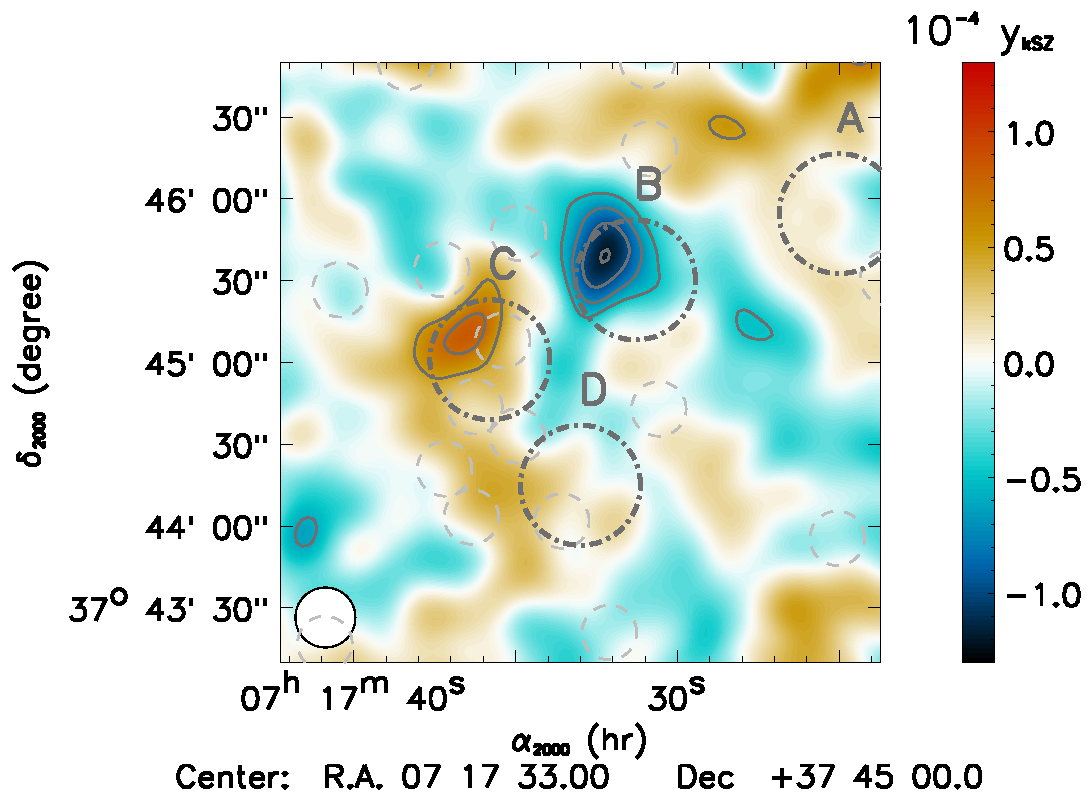
\includegraphics[width=0.49\textwidth]{Figures/NIKA2-SZ/MACSJ0717_kSZ_map.pdf}
  \hspace{4mm}
  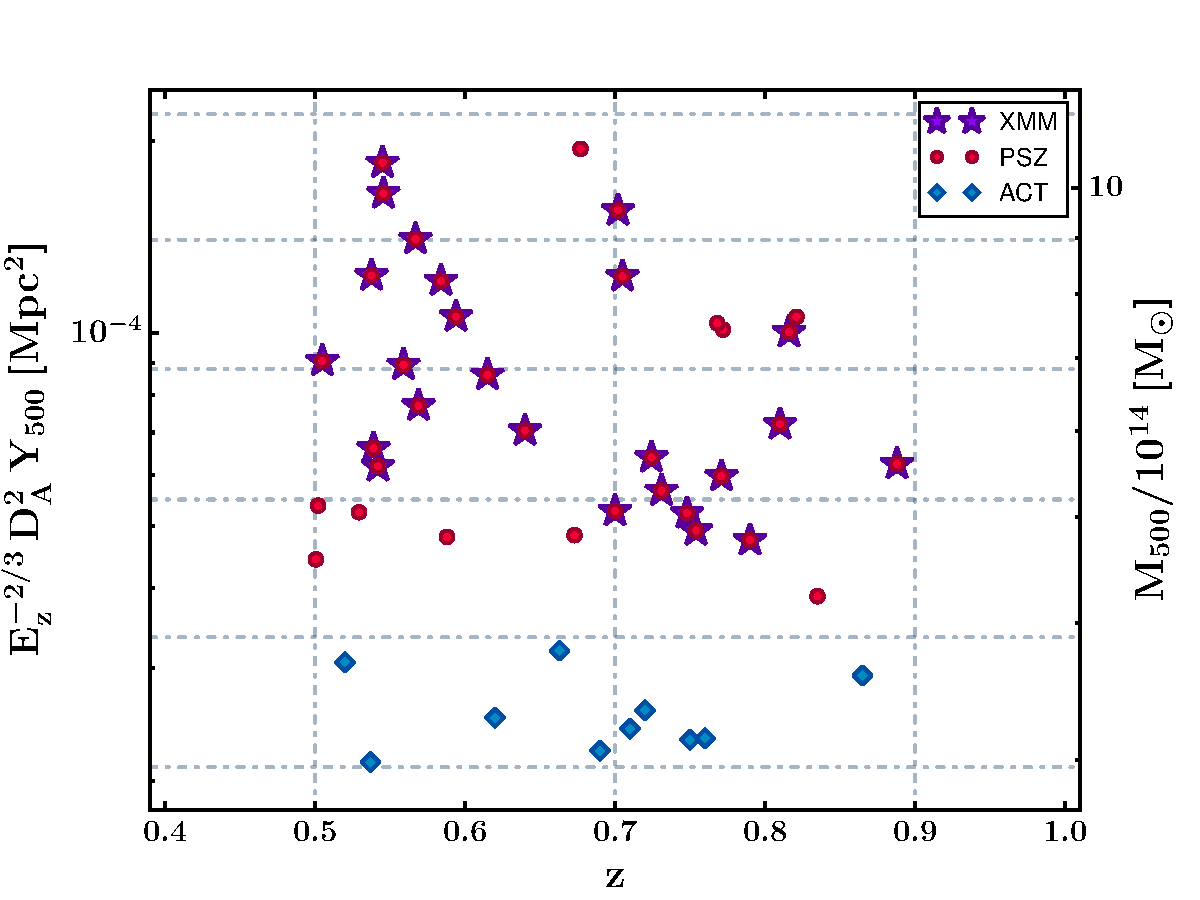
\includegraphics[width=0.44\textwidth, clip=true, trim=0cm -0.7cm 0cm 0cm]{Figures/NIKA2-SZ/LPSZ_M_z_grid.pdf}
  \caption{Left: Map of the kinetic SZ effect toward \mbox{MACS~J0717.5+3745} using NIKA pathfinder data, as discussed in Adam et al. (2017)$^{31}$. Right: NIKA2 Guaranteed-time cosmology program sample of galaxy clusters}
  \label{fig:nikanika2}
\end{figure}

\subsection{Premiers résultats de NIKA2}
{\color{vert}\lipsum[2-4]}

\begin{figure}
  \centering
  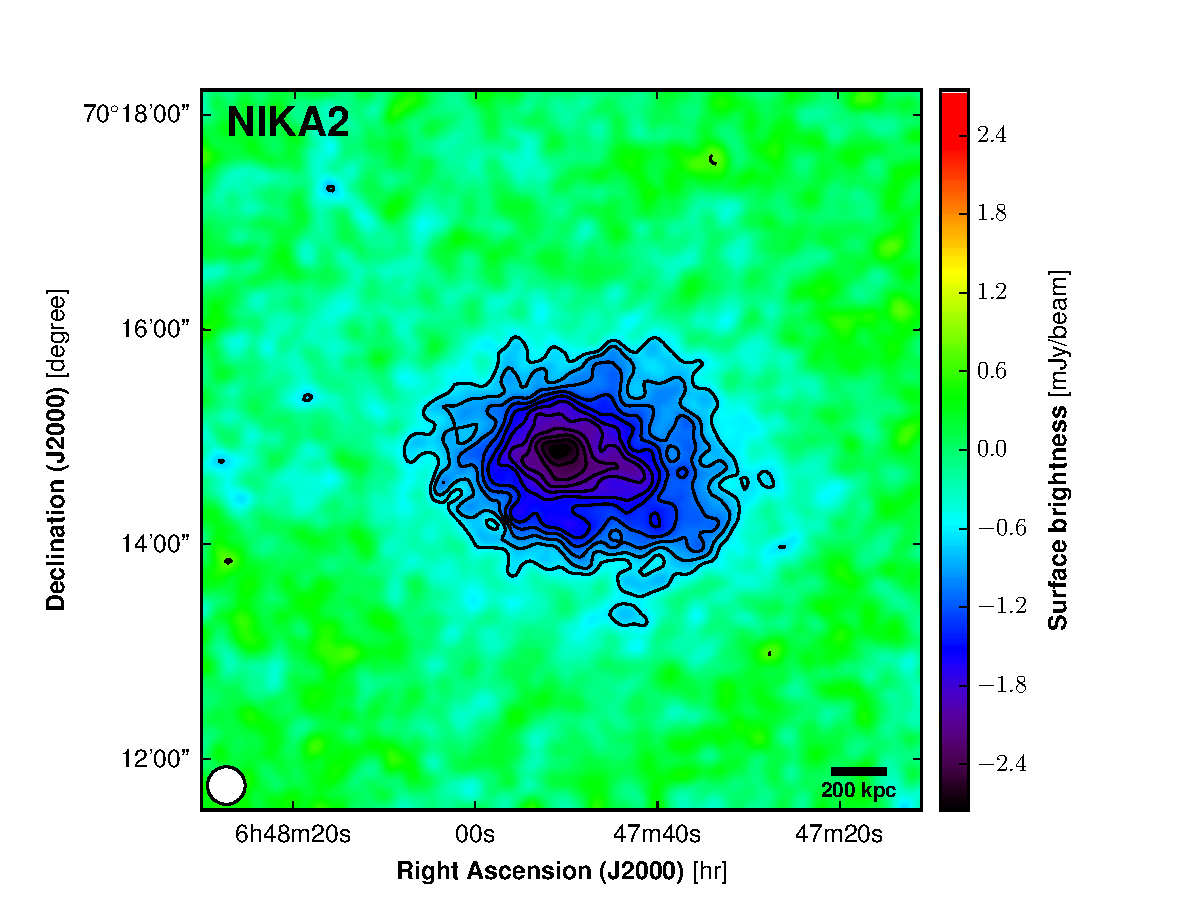
\includegraphics[width=0.49\textwidth]{Figures/NIKA2-SZ/Paper_NIKA2_Data.pdf}
  \includegraphics[width=0.44\textwidth]{Figures/NIKA2-SZ/Fig_PSZ2_G144_Scaling_relation.pdf}
  \caption{First SZ results with NIKA2. Left: The NIKA2 SZ map toward the galaxy cluster PSZ2-G0144.83+25.11. The high-resolution (20~arcsec) high-accuracy ($13.5\sigma $ measurement at peak) map covers the cluster from the core to the outskirts and reveals its morphology. An excess SZ signal is observed in the South-West region, indicating an overpressure within the intracluster medium (ICM). Right: Illustration of the impact of the ICM dynamics on the inner scatter of the SZ mass-observable relation. NIKA2 $Y_{500}$ estimates from the analysis with and without masking the over-pressure of PSZ2-G0144.83+25.11 are shown as a function of $M_{500}$, along with the cluster sample and the $Y_{500}-M_{500}$ scaling relation used in \emph{Planck} SZ-selected cluster count based cosmology analysis$^{13}$. These figures are extracted from Ruppin {\it et al.} (2018)$^{34}$. }
  \label{fig:nika2-sz}
\end{figure}



%----------------------------------------------------------------------------------------
%
%
%
%
%
%                 Prospectives ? 
%
%
%
%----------------------------------------------------------------------------------------
\section{Résultats attendus, implication pour la cosmologie et
  prospectives}


[Résultats principaux attendus] \\

[Amélioration des contraintes cosmologiques avec les amas de galaxies
  dasn Planck + pour les autres survey SZ]\\

[Etudes multisondes : contraintes sur le biais hydrostatic]\\

[synergie avec NOEMA]\\

[Calibration des futurs surveys optique/NIR]\\
